\chapter{The Single Skill That Built His \$100M Year Business}

This chapter follows a School of Hard Knocks interview, curated by LazyingArt LLC, but we can read it as a compact lecture on portability, feedback, and scale. Johnny Anton's central claim is that sales is not merely a job title; it is a transportable power that survives weak beginnings, unstable markets, and even the loss of capital. The displayed equations below are schematic rather than literal board formulas. They are used to keep track of the causal structure of the lecture: failure must be de-dramatized, imagination must be disciplined, action must be reviewed, and scale depends on borrowed pattern recognition as much as on personal effort.

\section{Portable Skill Under Market Uncertainty}

The opening minutes do not begin with tactics. They begin with authority and stakes. Anton is introduced as someone who helped scale multiple businesses to over nine figures in revenue, and that credential is immediately placed against a rougher background: an immigrant family from Iraq, poverty in Detroit, and two years of homelessness. The lecture wants us to see an asymmetry. Background is unstable, markets are unstable, and whole sectors can collapse. The skill of selling, however, is presented as unusually durable.

This is why the opening promise is so strong. The economy can crash, crypto can go down, fraud can appear, and yet a person who can sell a high-demand offer remains useful. We are meant to begin from that premise. The lecture is therefore not organized as generic motivation. It is organized as a theory of what remains when externals are stripped away.

\section{Failure, Time, and the Younger Self}

\subsection{Question \& Answer}

The first direct question asks what advice Anton would give his younger self. The answer is not a trick and not a list of business hacks. It is a rule for handling information: fail faster, and do not make the failure mean too much.

We can write the rule in the lecture's own causal spirit as
\begin{equation}
\text{Failure} + \text{Learning} + \text{Time} \to \text{Compounded Improvement}.
\end{equation}

The important word here is not merely \emph{failure}; it is \emph{time}. Anton's complaint is that people attach apocalyptic meaning to very small reversals. Once failure is over-signified, experimentation slows down, and time no longer compounds. He then enlarges the point by invoking Israel as an example of a culture of intelligent failing-forward. Whether or not we independently verify every numerical claim, the pedagogical function is clear: he wants the audience to see repeated, low-drama experimentation as an engine rather than as a wound.

So the first movement of the lecture removes psychological friction. We are not yet building; we are clearing the emotional obstruction that would prevent building.

\section{Meditation, Imagination, and the First Step}

Once failure has been stripped of excessive meaning, the lecture pivots inward. Anton is asked for the habits behind his success, and the first habit is not a spreadsheet, a call script, or a hiring plan. It is daily meditation. He describes this as reconditioning the mind, opening the subconscious to the conscious, and removing old limitations.

\begin{figure}[h]
\centering

\includegraphics[width=0.82\textwidth]{lecture_108_figure_02.png}
\caption{Anton's first numbered habit as it appears on screen: meditating every day.}
\end{figure}

The on-screen editorial label captures the structure of the moment:
\begin{equation}
\text{STEP 1: MEDITATING EVERYDAY}.
\end{equation}

Now the lecture widens this first step into a more ambitious claim. Anton says that manifestation begins in imagination. The Disney example is used precisely because it sounds implausible at first hearing: a fictitious amusement park, cartoon characters, adults and children, and large sums of capital asked for before the thing exists. He says that around 150 bankers said no, that the initial number was about \$5 million, and that the project ultimately cost \$15 million. The numbers matter because they convert vague self-help language into concrete entrepreneurial risk.

The cleanest schematic version of this movement is
\begin{equation}
\text{Imagination} \to \text{Thought} \to \text{Action} \to \text{Material Result}.
\end{equation}

That is not a literal formula spoken in the room, but it is the lecture's logic. One must first hold a form in the mind that is not yet visible in the material world. Meditation is then not a decorative wellness practice. It is presented as the daily discipline by which possibility is kept alive long enough to direct behavior.

\paragraph{Anecdote.}
Anton says he has meditated consistently for over six years, and that one early exposure came at a wrestling camp where athletes meditated every day on winning a state championship.

\paragraph{Claim.}
The first habit is daily meditation, aimed not at passivity but at the removal of old limits and the drawing in of abundance and possibility.

\paragraph{Mechanism.}
The mind must be reconditioned before later tactics can stick. Otherwise new information lands inside an old identity and is sabotaged from within.

\section{Feedback Loops and Borrowed Pattern Recognition}

The lecture does not stay inward for long. The second and third habits are explicitly operational. First, Anton insists on consistent action plus documentation. Then he insists on paying for access to people who already have the result.

We may summarize the second step as
\begin{equation}
\text{Action}_t + \text{Documentation}_t \to \text{Feedback Loop} \to \text{Pattern Recognition}.
\end{equation}

This is the point at which the lecture becomes more analytical. Anton says he asks his sales team to file end-of-day reports: who they spoke with, what the result of the call was, what worked, and what did not. But he immediately adds a more subtle condition. One must not track only what was said. One must track who one was being behind the words. That is why he insists that context matters more than content.

We can write the lecture's sharper claim as
\begin{equation}
\text{Context} > \text{Content}.
\end{equation}

A worked schematic example makes his point clearer. Anton says that two salespeople can be given the same script and still get different results. In that case the decisive variable is not the literal text.

\begin{align}
\text{Content}_A &= \text{Content}_B,\\
\text{Context}_A &\neq \text{Context}_B,\\
\text{Result}_A &\neq \text{Result}_B.
\end{align}

This is not the mathematics of a laboratory; it is the bookkeeping of performance. But it is still a real explanatory move. The script is held fixed. The outcome changes. Therefore the lecture directs our attention to delivery, state, framing, and timing.

We can also write the update rule for the daily review in a slightly more explicit form:
\begin{align}
\text{Log}_t &= (\text{contacts},\text{outcomes},\text{working patterns},\text{failed patterns}),\\
\text{Review}(\text{Log}_t) &\to \text{Pattern Recognition}_{t+1}.
\end{align}

The sports analogy serves the same purpose. Even winners must go back and study what happened in the game, and not merely celebrate the result. Winning can conceal error. Only review reveals the structure of performance.

The third step then extends this logic outward. If pattern recognition is valuable, the fastest way to obtain it is not always to discover it alone. One should pay people who already possess it.

\begin{equation}
\text{Proven Models} + \text{Paid Access} \to \text{Transferred Pattern Recognition}.
\end{equation}

\begin{figure}[h]
\centering
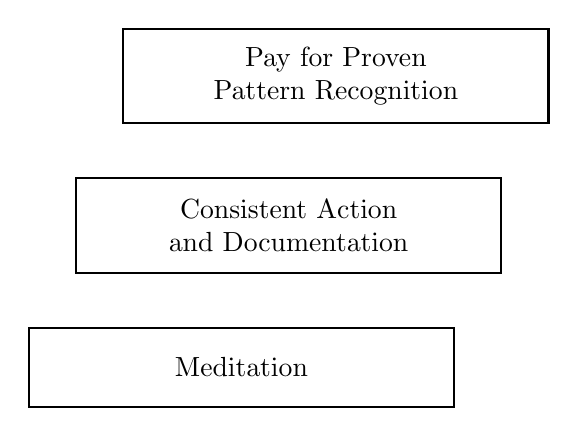
\begin{tikzpicture}
\draw[thick] (0,0) rectangle (5.4,1.0);
\node[align=center] at (2.7,0.5) {Meditation};

\draw[thick] (0.6,1.7) rectangle (6.0,2.9);
\node[align=center] at (3.3,2.3) {Consistent Action\\and Documentation};

\draw[thick] (1.2,3.6) rectangle (6.6,4.8);
\node[align=center] at (3.9,4.2) {Pay for Proven\\Pattern Recognition};
\end{tikzpicture}
\caption{A schematic reading of the three-step sequence developed in the interview.}
\end{figure}

The lecture later recaps these three pieces---meditation, consistent action with feedback, and modeled pattern recognition---and that recap is important. It tells us that Anton thinks of success not as a pile of disconnected traits, but as an ordered system: interior conditioning first, operational review second, borrowed leverage third.

\section{Founder Identity and the Problem of Scale}

\subsection{Question \& Answer}

Once the three-step architecture has been laid down, the lecture turns to a new obstruction. What if a person has energy, confidence, even visible success, and still builds badly? Anton's answer is direct: ego is not your friend.

The founder anecdote is concrete. His boss, Paul, asked whether he was really ready to give up roughly \$500{,}000 in one-hundred-percent commission sales income, especially since that income required no marketing, no delivery risk, no hiring, no operations, and no finance burden. Anton's younger answer was that it could not be that hard. He had helped scale a company, built training, action plans, sales processes, advanced scripting, and storytelling, and at age twenty-four he believed he could easily dominate the next stage.

\paragraph{Anecdote.}
He describes himself as arrogant in his twenties, convinced that previous performance automatically entitled him to founder-level success.

\paragraph{Claim.}
The missing move is not more confidence but surrender of the old identity.

\paragraph{Mechanism.}
The ego wants control, wants originality, and wants to prove itself. That makes it allergic to the very thing the lecture has already recommended, namely paying for proven models and submitting to them.

This is why the founder section belongs exactly here in the lecture. Without it, the earlier habits could sound like neutral productivity advice. With it, we see the deeper point: information is often not scarce; obedience to better models is scarce.

The lecture then widens from founder psychology to firm structure. Anton says that what takes a business from seven to eight figures, and then eight to nine, comes down to fundraising and recruiting. He introduces Ryan Breslow as an example of a very young founder building multiple multi-billion-dollar companies, and he extracts two structural levers from that example.

We can write Anton's scale-chain as
\begin{equation}
\text{Product} \to \text{Leadership} \to \{\text{Recruiting},\ \text{Fundraising}\} \to \text{Scale}.
\end{equation}

The logic is not that money alone scales a company. A strong product is needed to attract strong leaders. Strong leaders enable recruiting and fundraising. Those in turn supply the talent and cash required for growth. Later Anton sharpens the argument further by saying that top-tier talent in technology is decisive, that companies steal talent from one another, and that compensation packages depend on a product strong enough to sell itself.

\section{Rebuilding from Zero and Structuring the Sale}

\subsection{Question \& Answer}

The interview now asks a clean stress-test question: if the bank account went to zero tomorrow, what would be the first step? Anton's answer is wonderfully unromantic. Go sell the most expensive thing available until rent is paid.

The lecture then introduces a stripped-down human sequence. First food and shelter, then belonging, then actualization. Anton explicitly invokes Maslow's hierarchy here, not as academic psychology, but as a reminder that empire-building is downstream of basic stability.

\begin{equation}
\text{Food \& Shelter} \to \text{Belonging} \to \text{Actualizing Potential}.
\end{equation}

Once the floor is secured, the rebuild becomes sequential. Add value for free, gather testimonials and case studies, land an anchor client, move into adjacent competitors and nearby niches, then build a team and widen lead sources.

\begin{equation}
\text{Free Value} \to \text{Testimonials/Case Studies} \to \text{Anchor Client} \to \text{Sales Team} \to \text{Ads \& Lead Sources}.
\end{equation}

This is perhaps the most explicit algorithm in the lecture. It can be read as a worked entrepreneurial construction:

\begin{enumerate}
\item Restore immediate cash by selling a high-ticket offer.
\item Stabilize life at the level of food and shelter.
\item Create social proof through unpaid value.
\item Convert proof into an anchor client.
\item Expand outward from that anchor into a cluster of related buyers.
\item Only then add sales infrastructure and paid lead generation.
\end{enumerate}

What is striking is that Anton refuses to mystify the early stage. He does not begin with branding language or grand identity statements. He begins with survival, proof, adjacency, and scale.

\subsection{Question \& Answer}

The final technical question is how to turn a no into a yes. Anton's answer is to reject the framing. If we wait until the objection arrives, we are already too late. The sale should have been structured earlier.

He therefore defines sales as
\begin{equation}
\text{Current Situation} \xrightarrow{\text{transfer of certainty}} \text{Desired Situation}.
\end{equation}

This definition matters because it replaces manipulation with translation. The seller is not supposed to force an alien outcome on the buyer. The seller is supposed to understand the buyer's present state, understand the buyer's desired state, and make credible the bridge between them.

That is why the lecture ends with demographics and psychographics. Demographics tell us who the person is in broad profile. Psychographics tell us what the person wants, fears, values, and how the person decides. Only when both are understood can we solve the actual problem on the phone.

The last schematic line of the chapter is therefore
\begin{equation}
\text{Demographics} + \text{Psychographics} \to \text{Problem Understanding} \to \text{Objection Prevention}.
\end{equation}

We can state the logic in steps:
\begin{enumerate}
\item Identify the prospect's current condition.
\item Identify the prospect's desired condition.
\item Understand the profile and decision psychology of the prospect.
\item Frame the offer as the bridge across that gap.
\item Block foreseeable objections in the presentation rather than trying to rescue the close at the very end.
\end{enumerate}

The lecture closes where it began: sales is treated as a deep, portable craft. The person who can understand desire, remove friction, and transfer certainty holds a tool that remains useful long after particular markets rotate.

\section{Summary}

The chapter unfolds as a sequence rather than a slogan. First we strip failure of melodrama so that time can compound learning. Then we discipline imagination through meditation so that thought can take stable form. Then we add feedback, review, and borrowed pattern recognition so that action becomes increasingly intelligent. After that the lecture turns to founder identity, where ego and attachment to control become the real obstacles to scale. Finally it shows how scale depends on product, leadership, recruiting, and fundraising, and how a person starting from zero rebuilds through value creation, proof, and a properly structured sale.

If we want the shortest faithful summary, it is this: Anton treats sales as a transportable engine of wealth, but only when it is joined to three deeper disciplines---psychological de-dramatization, operational feedback, and humble submission to proven patterns.